\documentclass[10pt]{article}
\usepackage{sdss2020} % Uses Times Roman font (either newtx or times package)
\usepackage{url}
\usepackage{latexsym}
\usepackage{amsmath, amsthm, amsfonts}
\usepackage{algorithm, algorithmic}  
\usepackage{multirow,graphicx}
\usepackage[flushleft]{threeparttable}
\usepackage[T1]{fontenc}
\graphicspath{ {./images/} }

\title{Modeling Opening Weekend Revenue for U.S. Box Office Movies, 2005-2007}

\author{
  C. Logue \\
  Georgetown University \\
  Washington, DC \\
\\\And
  P. Mernagh \\
  Georgetown University \\
  Washington, DC \\
\\\And
  Z. Holden \\
  Georgetown University \\
  Washington, DC \\
\\}

\begin{document}
\maketitle

\section{Introduction}
The project objective is to predict as accurately as possible opening weekend box office revenue for a set of movies, specifically from 2005-2007. Motivation for this project is a wealth of data points from both The Movie Database (TMDB) and Internet Movie Database (IMDb) around historical movies and TV shows: user-submitted ratings, applicable genres, budget, release date, actors, producer(s), production companies, country (or countries) of origin, etc. Further motivation is a prior understanding of likely useful predictors, such as the movie's budget, or the seasonal factors affecting a movie release. For example, the periods January-February, and to a lesser extent August-September, have been referred to as the ``dump months, '' i.e. effectively a dumping ground for low-potential movies that are not expected to make as much money. Various factors such as the seasonality of consumer spending (i.e binge before the holidays, pay down debt later), the timing of Golden Globes and Oscars awards, weather, the Super Bowl, and vacation months may all lead to seasonality in box office receipts.  The years 2005-2007 were specifically chosen since they predate the rise of the streaming era and its potential impacts on box office sales. They are a short enough period that no inflation adjustment is made to any financial variables. 
\section{Data}

Data on approximately 500 movies that opened in U.S. theaters between 2005-2007 was aggregated from TMDB and IMDb. Only English-language movies are included. Retrieved data points include the release date, the opening weekend revenue, budget, and the number of theaters the movie opened in. A selection of genres that each movie could be classified as (e.g. drama, thriller, action, crime, documentary, etc.) is included. Most movies are tagged with two to three genres, though a handful go as high as six. Popularity, a proprietary TMDB metric, is also included. It itself is based on various data points including votes, views, release date, etc.. As a community-built database, TMDB provides the data point vote average, namely the mean of user-submitted ratings on the scale of 0-10, as well as the number of submitted votes.  Both the origin and production country (or countries) are included. The production companies are provided (e.g big hitters such as Paramount, Warner Bros, MGM). Finally, the runtime, and what collection the movie belongs to, if any, such as the Harry Potter series or the Pirates of the Caribbean collection. The operating revenue and number of opening theaters were specifically pulled from Box Office Mojo, a service of IMDB Pro. The following predictors are chosen for initial modeling:
\begin{enumerate}
\item Budget (continuous)
\item Runtime (continuous)
\item Number of production companies (continuous)
\item From a series (binary, 118 total)
\item Opening weekend season (categorical)
\begin{enumerate}
\item Winter: January-February (71 total)
\item Spring: March-April (84 total)
\item Summer: May-August (154 total)
\item Fall: September-October (120 total)
\item Holiday: November-December (82 total)
\end{enumerate}
\end{enumerate}

Summary statistics are as follows:
\begin{table}[H]
\centering
\caption{Summary Statistics (n = 511)}
\begin{tabular}{|lrrr|} 
\hline
Variable & Mean & Min & Max \\ 
\hline
opening revenue (\$) & 14,743,982 & 9,653 & 151,116,516\\
\hline
budget (\$) & 40,365,469 & 0 & 300,000,000\\
\hline
runtime (min) & 107 & 14 & 187\\
\hline
\# of prod. cos. & 3.8 & 0 & 17\\
\hline
\end{tabular}  
\end{table}

The variable popularity is not considered, since it is modeled by TMDB and likely influenced by post-opening weekend factors. The number of theaters the movie opened in is likely highly correlated with opening revenue. However, the project prefers variables that are intrinsic characteristics of a movie, thus number of theaters is also not considered further. 

A secondary set of variables, intended for follow-up modeling, is also aggregated or created via transformation. These include data points around the production room, writers room, sound room, and crew. Additionally, data around the credits and median rating is provided for producers, writers, and leads. A binary variable for whether the movie is based on a novel is included. An indie binary variable is created based on whether the movie was produced by a major production company or by a smaller (indie) company. Finally, indicator variables for the following genres are created: adventure, fantasy, animation, drama, horror, action, comedy, history, western, thriller, crime, documentary, science fiction, mystery, music, romance, family, and war.

\section{Methods}
First, the relationships between the initial selected predictors are visually examined. From pair plots of the continuous predictors (Figure 1), budget and opening revenue seem positively, linearly related. There is no apparent relationship between opening revenue and the number of production companies or the runtime of the movie. 

For the non-continous predictors, the Spring, Summer, and Holiday seasons are associated with higher opening revenue on average (Figure 2), though this is skewed, especially by releases grossing over \$50M. Movies that are part of a series also are associated with higher opening revenue on average (Figure 3). 

Armed with this knowledge, various models are fit to the data. Initially, a model incorporating all variables produces $R^2_a$ of over 60\%, but demonstrates clear heteroskedasticity of residuals. A square-root transformation noticeably stabilizes the variance. After this transformation, the initial best model candidate is:

\begin{table}[H]
  \begin{threeparttable}
    \caption{Initial Model Specification}
       \begin{tabular}{|l l l l l|} 
	 \hline
	 & Coef & 95\% CI & t-stat & p-value \\ [0.5ex] 
	 \hline
	intercept & 2006.7 & [1810.3, 2203.1] & 20.075 & <0.0001 \\ 
	\hline
	budget & 2.96e-05 & [2.67e-05, 3.25e-05] & 20.020 & <0.0001\\
	 \hline
	is\_series & 1379.9 & [1088.4, 1671.5] & 9.298 & <0.0001\\
	\hline
	is\_fall & -795.2 & [-1085.1, -505.4] & -5.390 & <0.0001\\
	\hline
	is\_holiday & -729.1 & [-1063.7, -394.5] & -4.281 & <0.0001\\[1ex]
	\hline
      \end{tabular}
    \begin{tablenotes}
      \small
      \item $R^2_a$ = 0.58
    \end{tablenotes}  
  \end{threeparttable}    
\end{table}

Backwards elimination:


\section{Results}

\section{Discussion}

\bibliographystyle{sdss2020} 
%\bibliography{fullbib}

\appendix

\section{Visualizations}
\begin{figure}[H]
	\begin{center}
		\centerline{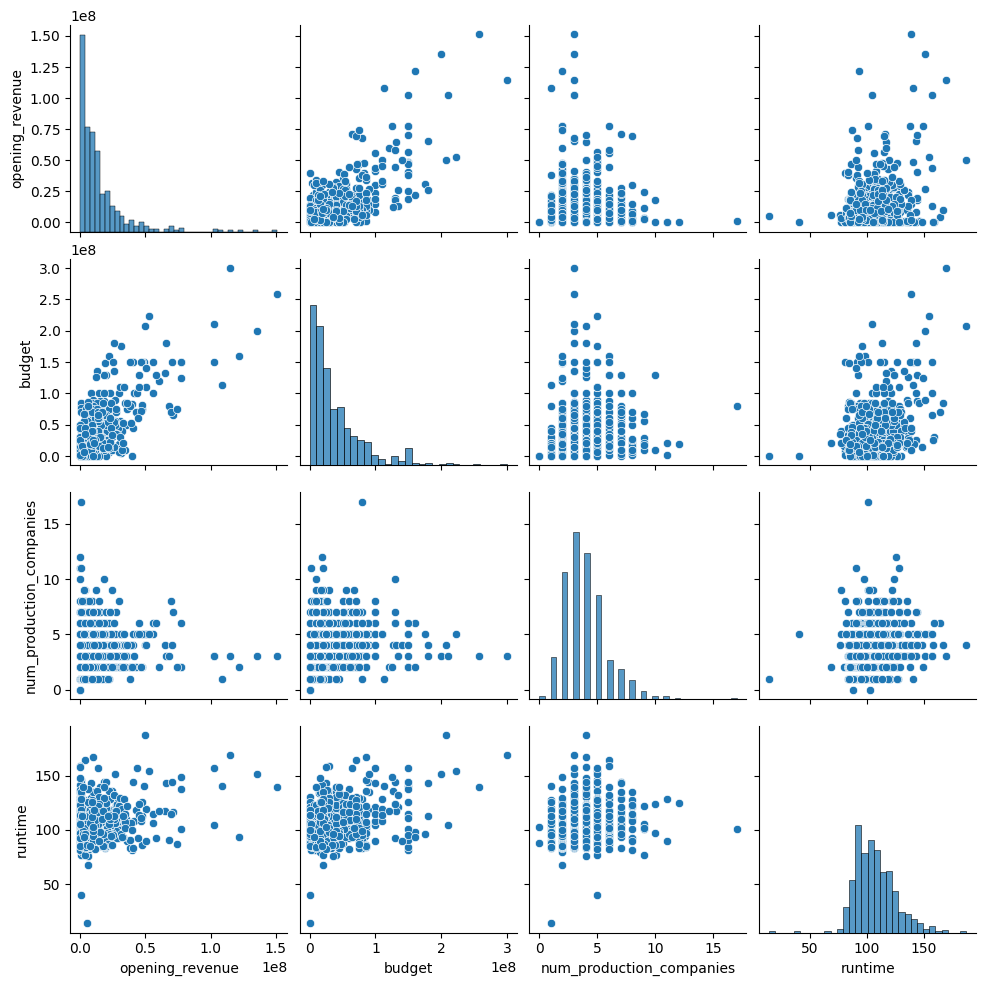
\includegraphics[width=\columnwidth]{pairs_plot}}
		\caption{Pairs plot, initially selected continuous variables.}
	\end{center}
\end{figure}

\begin{figure}[H]
	\begin{center}
		\centerline{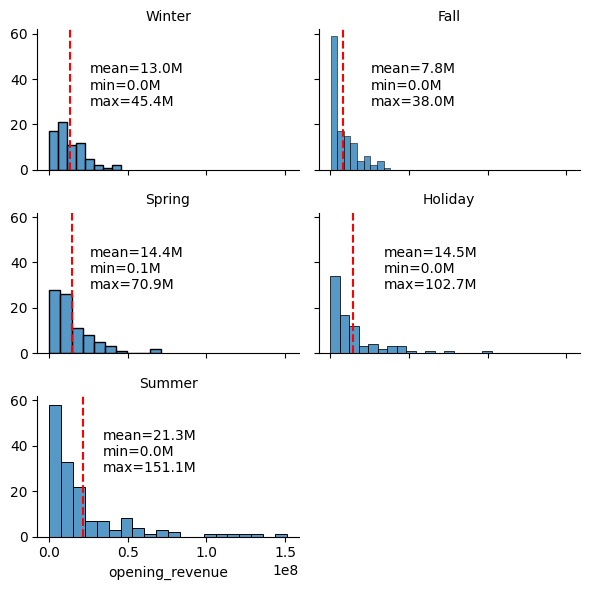
\includegraphics[scale=0.5]{season_revenue}}
		\caption{Distribution of opening revenue by season}
	\end{center}
\end{figure}

\begin{figure}[H]
	\begin{center}
		\centerline{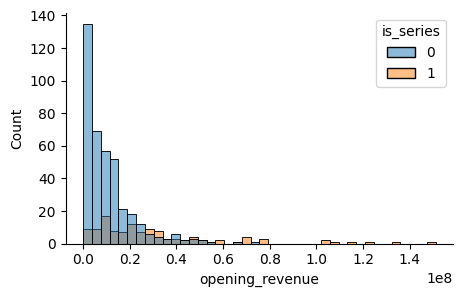
\includegraphics[scale=0.6]{is_series}}
		\caption{Distribution of opening revenue, series vs. non-series}
	\end{center}
\end{figure}

\begin{figure}[H]
	\begin{center}
		\centerline{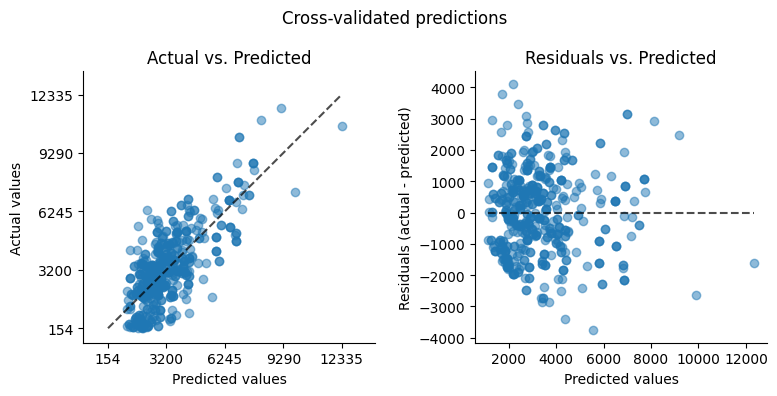
\includegraphics[width=\columnwidth]{cross_val}}
		\caption{Cross-validation prediction results.}
	\end{center}
\end{figure}

\begin{figure}[H]
	\begin{center}
		\centerline{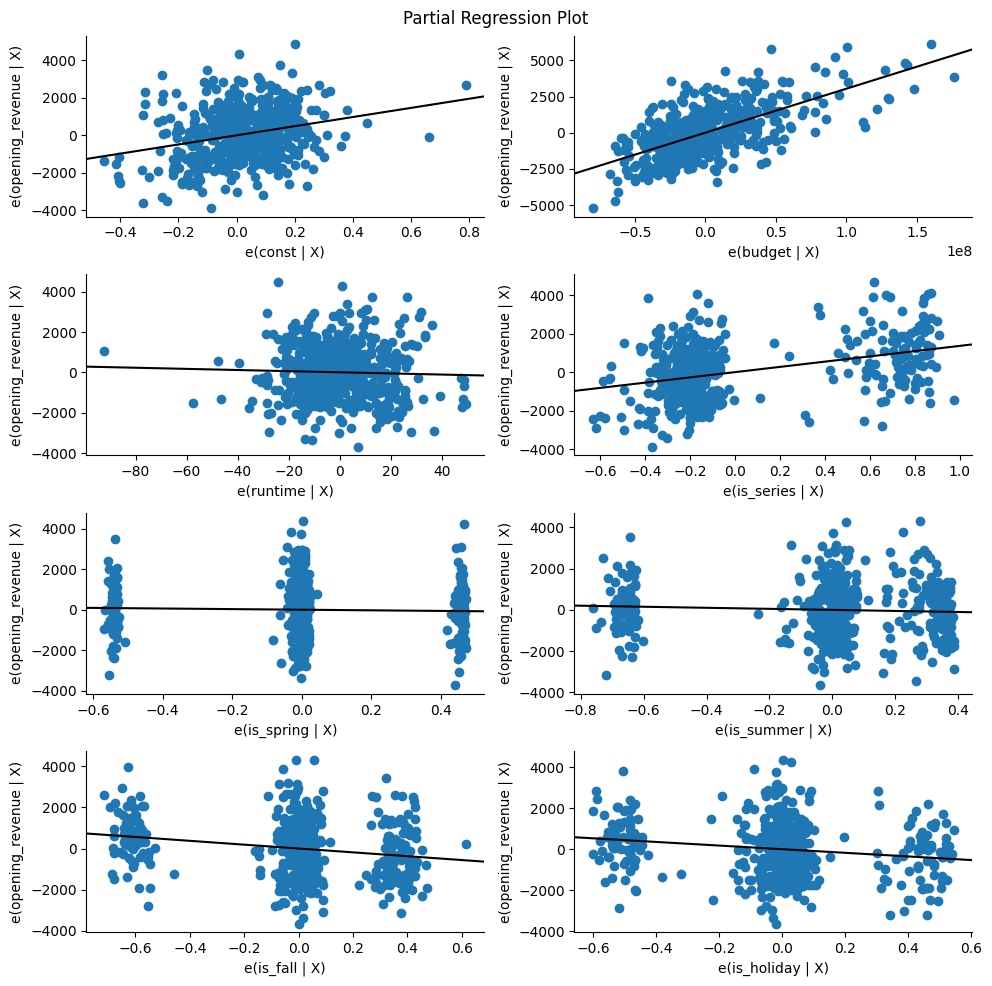
\includegraphics[width=\columnwidth]{partial_regression}}
		\caption{Partial Regression Plots}
	\end{center}
\end{figure}

\section{Replication Data and Code}
\label{a:code}
The repo \mbox{https://github.com/cons-code/MATH-5500} contains replication data and code.
\end{document}